
\chapter{Descrição do Repositório}

\label{Anexo-Repositorio}

O \textit{link} de acesso do repositório é ``https://github.com/rafael-at97/WMRA-UnB''. A 
oganização do mesmo, indicando principais arquivos e diretórios pode ser vista na figura
\ref{fig:repositorio}.

\begin{figure}[h]
    \caption{Organização do respositório.}    

    \begin{centering}
        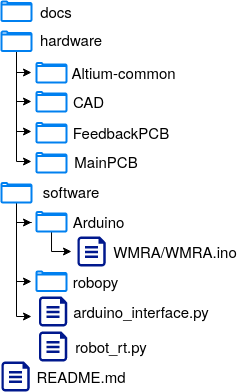
\includegraphics[width=0.3\columnwidth]{images/anexo/repositorio.png} 
    \par\end{centering}

    \label{fig:repositorio}
\end{figure}

Todos os arquivos necessários para a criação deste documento estão dentro da pasta `\textit{docs}',
os arquivos de texto estão no formato LATEX.

A pasta \textit{hardware} agrupa todos os arquivos relacionados a partes físicas do projeto,
como as bibliotecas desenvolvidas para representar circuitos eletro-eletrônicos criadas
durante o projeto dos circuitos, pasta `\textit{Altium-common}', documentos do projeto das 
placas em si, pastas `\textit{FeedbackPCB}' e `\textit{MainPCB}' e o modelo 3D do manipulador, na 
pasta `\textit{CAD}'.

Já o que foi desenvolvido em relação a partes lógicas do sistema estão dispostos dentro da pasta
`\textit{software}'. Na pasta `Arduino' encontram-se todas as bibliotecas desenvolvidas para o 
sistema embarcado e o código principal utilizado para o controle geral do sistema, denominado
por `WMRA/WMRA.ino'. A pasta `\textit{robopy}' faz alusão a outro repositório, também criado pelo
autor deste documento, que organiza as interpretações das funções da \textit{toolbox} de robótica
para MATLAB, mas em uma versão escrita em \textit{python}. O código `\textit{arduino\_interface.py}'
realiza a interface entre os dados vindos do arduino e o módulo de simulação. A criação da representação
do manipulador utilizando os módulos desenvolvidos está no arquivo `\textit{robot\_rt.py}', que tenta 
realizar a atualização do modelo em tempo real, ou \text{real-time}.

Por fim, há um arquivo `\textit{README.md}', que fornece informações básicas sobre o projeto.
